\documentclass[14pt,aspectratio=169]{beamer}

\usepackage{pgfpages}
\usepackage{fancyvrb}
\usepackage{pgfplots}

\usepackage{minted}
\usemintedstyle{tango}

\usepackage{amsfonts}

\usepackage{moresize}
\usepackage{anyfontsize}

\usepackage{tikz}
\usetikzlibrary{arrows,shapes}
\usetikzlibrary{arrows.meta}

\tikzstyle{process}=[rectangle, draw, thick, text width=5em, text centered, minimum height=2.5em, fill=gray!40]
\tikzstyle{entity}=[rounded rectangle, draw, thick, text width=5em, text centered, minimum height=1.5em, fill=gray!40]

\usetheme{auriga}
\usecolortheme{auriga}

\setbeamercolor{background canvas}{bg=lightgray}

% define some colors for a consistent theme across slides
\definecolor{red}{RGB}{181, 23, 0}
\definecolor{blue}{RGB}{0, 118, 186}
\definecolor{gray}{RGB}{146, 146, 146}

\title{Discrete Structures: \\ Functions and Expressions in the Python Language}

\author{{\bf Gregory M. Kapfhammer}}

\institute[shortinst]{{\bf Department of Computer Science, Allegheny College}}

\begin{document}

{
  \setbeamercolor{page number in head/foot}{fg=background canvas.bg}
  \begin{frame}
    \titlepage
  \end{frame}
}

%% Slide
%
\begin{frame}{Technical Question}
  %
  \begin{center}
    %
    {\large How do I use non-recursive functions, recursive functions, and
    lambda expressions to perform mathematical operations such as computing the
  absolute value of a number and the mean and median of a sequence of numbers?}
    %
  \end{center}
  %
  \vspace{2ex}
  %
  \begin{center}
    %
    \small Let's learn how to use the Python programming language to different
    types of functions that perform mathematical and statistical computations!
    %
  \end{center}
  %
\end{frame}

% Slide
%
\begin{frame}{Python Programming with Functions}
  %
  \begin{itemize}
    %
    \item Intuitively read the functions to grasp their behavior
      %
      \vspace*{-.15in}
      %
    \item Key components of the Python functions
      %
      \begin{itemize}
        %
        \item Definition of the function
          %
        \item Parameter(s) that serve as the input
          %
        \item Body that performs a computation
          %
        \item Function return value(s) that produce output
          %
        \item Invocation of the function
          %
        \item Collecting the output of the function
          %
        \item Test case(s) for the function
          %
      \end{itemize}
      %
      \vspace*{-.2in}
      %
    \item Investigate the ways to {\em define} and {\em call} Python functions!
      %
  \end{itemize}
  %
\end{frame}

% Slide
%
\begin{frame}[fragile]
  \frametitle{Computing the Absolute Value of a Number}
  \normalsize
  \hspace*{-.65in}
  \begin{minipage}{6in}
    \vspace*{.25in}
    \begin{minted}[mathescape, numbersep=5pt, fontsize=\large]{python}
    def abs(n):
        if n >= 0:
            return n
        else:
            return -n
    \end{minted}
  \end{minipage}
  \vspace*{.25in}
  \begin{center}
    %
    \normalsize \noindent The absolute value of a number is its distance from zero \\
    \normalsize \noindent What is the output of {\tt print(str(abs(10)))}? \\
    \normalsize \noindent What is the output of {\tt print(str(abs(-10)))}? \\
    %
  \end{center}
  %
\end{frame}

% Slide
%
\begin{frame}[fragile]
  \frametitle{Alternative Absolute Value Computation}
  \normalsize
  \hspace*{-.65in}
  \begin{minipage}{6in}
    \vspace*{.25in}
    \begin{minted}[mathescape, numbersep=5pt, fontsize=\large]{python}
    def abs(n):
        if n >= 0:
            return n
        return -n
    \end{minted}
  \end{minipage}
  \vspace*{.25in}
  \begin{center}
    %
    \normalsize \noindent Does this function compute the same value? \\
    \normalsize \noindent Which implementation of {\tt abs} do you prefer? \\
    \normalsize \noindent Which implementation of {\tt abs} does {\tt pylint} prefer? \\
    \normalsize \noindent There are different ways to implement the same function! \\
    %
  \end{center}
  %
\end{frame}

% Slide
%
\begin{frame}[fragile]
  \frametitle{Using Newton's Method in a Function}
  \hspace*{-.8in}
  \begin{minipage}{6in}
    \begin{minted}[mathescape, numbersep=5pt, fontsize=\large]{python}
    def sqrt(num: int, tol: float):
        guess = 1.0
        while abs(num - guess*guess) > tol:
            guess = guess -
            (guess*guess - num)/(2*guess)
        return guess
    \end{minted}
  \end{minipage}
  \vspace*{.05in}
  \begin{center}
    %
    \normalsize \noindent What are the benefits of defining this as a function? \\
    \normalsize \noindent What is the meaning of ``{\tt num:int}'' and ``{\tt tol:float}''? \\
    %
  \end{center}
\end{frame}

% Slide
%
\begin{frame}{Reminders About Industry-Standard Python}
  %
  \begin{itemize}
    %
    \item Please use Python 3 for all of your programs!
      %
      \vspace*{-.15in}
      %
    \item Add ``docstring'' comments to your Python programs
      %
      \begin{itemize}
        %
        \item Module
          %
        \item Class
          %
        \item Function
          %
      \end{itemize}
      %
      \vspace*{-.2in}
      %
    \item Add comments for important blocks of your function
      %
      \vspace*{-.2in}
      %
    \item Use descriptive variable and function names
      %
      \vspace*{-.2in}
      %
    \item Use type hints to explain the type of each parameter
      %
  \end{itemize}
  %
\end{frame}

% Slide
%
\begin{frame}[fragile]
  \frametitle{Recursive Functions in Python Programs}
  \hspace*{-.8in}
  \begin{minipage}{6in}
    \begin{minted}[mathescape, numbersep=5pt, fontsize=\large]{python}
    def factorial(number: int):
        if number == 1:
            return 1
        return number * factorial(number - 1)

    num = 5
    print("The factorial of " + str(num) +
           " is " + str(factorial(num)))
    \end{minted}
  \end{minipage}
  \vspace*{.05in}
\end{frame}

% Slide
%
\begin{frame}{Recursive Computation of the Factorial Function}
  %
  \begin{itemize}
    %
    \item As an equation: $n! = n \times n-1 \times n-2 \times \ldots \times 1$
      %
      \vspace*{-.15in}
      %
    \item What are the parts of a recursive function in Python?
      %
      \begin{itemize}
        %
        \item Defined by cases using conditional logic
          %
        \item A function definition that calls itself
          %
        \item A recursive call that makes progress to a base case
          %
        \item A base case that stops the recursive function calls
          %
      \end{itemize}
      %
      \vspace*{-.2in}
      %
    \item Repeatedly perform an operation through function calls
      %
      \vspace*{-.2in}
      %
    \item What would happen if you input a negative number?
      %
      \vspace*{-.2in}
      %
    \item How could you write this function with iteration?
      %
  \end{itemize}
  %
\end{frame}

% Slide
%
\begin{frame}[fragile]
  \frametitle{Finding the Parts of a Recursive Function}
  \hspace*{-.8in}
  \begin{minipage}{6in}
    \begin{minted}[mathescape, numbersep=5pt, fontsize=\large]{python}
    def factorial(number: int):
        if number == 1:
            return 1
        return number * factorial(number - 1)

    num = 5
    print("The factorial of " + str(num) +
           " is " + str(factorial(num)))
    \end{minted}
  \end{minipage}
  \vspace*{.05in}
\end{frame}

% Slide
%
\begin{frame}[fragile]
  \frametitle{Higher-Order Functions in Python}
  \hspace*{-.6in}
  \begin{minipage}{6in}
    \begin{minted}[mathescape, numbersep=5pt, fontsize=\large]{python}
    def square(number: int):
        return number * number

    def call_twice(f, number: int):
        return f(f(number))

    number = 5
    result = call_twice(square, number)
    \end{minted}
  \end{minipage}
  \vspace*{.05in}
\end{frame}

% Slide
%
\begin{frame}{Understanding Higher-Order Functions}
  %
  \begin{itemize}
    %
    \item You can pass a function as an argument to a function!
      %
      \vspace*{-.15in}
      %
    \item The behavior of higher-order functions in Python
      %
      \begin{itemize}
        %
        \item {\bf Step 1}: {\tt square} is a function that computes and
          returns $x^2$
          %
        \item {\bf Step 2}: {\tt call\_twice} is a function that calls a
          function {\tt f} twice
          %
        \item {\bf Step 3}: First, {\tt call\_twice} calls {\tt f} with {\tt
          number}
          %
        \item {\bf Step 4}: Then, {\tt call\_twice} calls {\tt f} with {\tt
          f(number)}
          %
        \item {\bf Step 5}: Finally, {\tt call\_twice} returns result of {\tt
          f(f(number))}
          %
      \end{itemize}
      %
      \vspace*{-.2in}
      %
    \item Can you predict the output of the {\tt call\_twice} function? How
      would you test the {\tt call\_twice} function? Can you express this
      computation in a different fashion?
      %
  \end{itemize}
  %
\end{frame}

% Slide
%
\begin{frame}[fragile]
  \frametitle{Calling Higher-Order Functions in Python}
  \hspace*{-.1in}
  \begin{minipage}{6in}
    \begin{minted}[mathescape, numbersep=5pt, fontsize=\large]{python}
num = 5
result = call_twice(square, num)
print("Calling the square twice with " +
      str(num) + " is " + str(result))
num = 5
result = num ** 4
print("Computation of twice square is "
      + str(num) + " is " + str(result))
    \end{minted}
  \end{minipage}
  \vspace*{.05in}
\end{frame}

% Slide
%
\begin{frame}[fragile]
  \frametitle{Lambda Expressions in Python}
  \hspace*{-.1in}
  \begin{minipage}{6in}
    \begin{minted}[mathescape, numbersep=5pt, fontsize=\large]{python}
square = lambda x: x*x
num = 5
result = call_twice(square, num)
print("Calling square lambda twice " +
      "with " +
      str(number) +
      " is " +
      str(result))
    \end{minted}
  \end{minipage}
  \vspace*{.05in}
\end{frame}

% Slide
%
\begin{frame}{Understanding Lambda ``Functions''}
  %
  \begin{itemize} \vspace*{-.2in}
    %
    \item You can define a ``function'' without an explicit name!
      %
      \vspace*{-.2in}
      %
    \item What are benefits of {\tt square = lambda x: x*x}?
      %
      \vspace*{-.2in}
      %
    \item What are drawbacks of {\tt square = lambda x: x*x}?
      %
      \vspace*{-.2in}
      %
    \item How do you decide between an ``anonymous'' and a ``named'' functions
      when implementing a computation?
      %
      \vspace*{-.2in}
      %
    \item How do you test a lambda function in a Python program?
      %
      \vspace*{-.2in}
      %
    \item Implement $n! = n \times n-1 \times n-2 \times \ldots \times 1$ as
      lambda?
      %
      \vspace*{-.2in}
      %
  \end{itemize}
  %
\end{frame}

% Slide
%
\begin{frame}{Creating Functions for Statistical Analysis}
  %
  \begin{figure}
    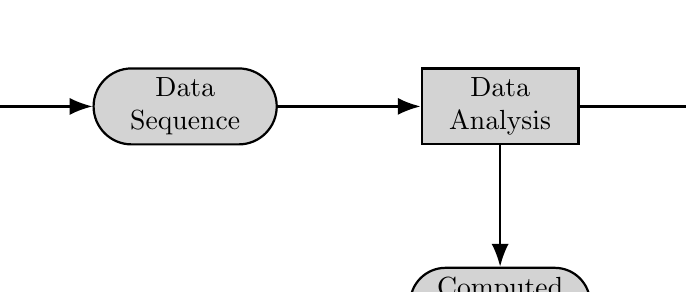
\begin{tikzpicture}[node distance=4cm, auto,>=latex', thick]
      %
      \path[use as bounding box] (2,1) rectangle (10,-2);
      %
      % Sensor* --> Data Sequence*
      %
      \path[->] node[process, font=\large] (sensor) {Sensor};
      \path[->] node[entity, right of=sensor, align=center] (values) {Data \\ Sequence};
      \path [draw, thick, -{>[scale=1.25]}, >=Latex] (sensor.east) -- (values.west);
      %
      % Data Sequence --> Data Analysis*
      %
      \path[->] node[process, right of=values, align=center] (analyze) {Data \\ Analysis};
      \path [draw, thick, -{>[scale=1.25]}, >=Latex] (values.east) -- (analyze.west);
      %
      % Data Analysis --> Computed Mean*
      %
      \path[->] node[entity, below of=analyze, align=center, yshift=1.5cm]
        (average) {Computed \\ Mean};
      \path [draw, thick, -{>[scale=1.25]}, >=Latex] (analyze.south) -- (average.north);
      %
      % Data Analysis --> Data Visualization*
      %
      \path[->] node[entity, right of=analyze, align=center] (graph) {Data \\ Graph};
      \path [draw, thick, -{>[scale=1.25]}, >=Latex] (analyze.east) -- (graph.west);
      %
    \end{tikzpicture}
    %
    \vspace*{.6in}
    \begin{center}
      %
      \normalsize
      %
      \noindent How do we compute the {\em mean} of a list of numbers? \\
      \noindent How do we compute summary statistics of a list of numbers? \\
      \noindent What type of function? Recursive? Iterative? Lambda?
      %
    \end{center}
    %
  \end{figure}
  %
\end{frame}

% Slide
%
\begin{frame}[fragile]
  \frametitle{Computing the Arithmetic Mean in Python}
  \hspace*{-.1in}
  \begin{minipage}{6in}
    \begin{minted}[mathescape, numbersep=5pt, fontsize=\large]{python}
def compute_mean(numbers):
    s = sum(numbers)
    N = len(numbers)
    mean = s / N
    return mean

numbers = [5,1,7,99,4]
print(str(compute_mean(numbers)))
    \end{minted}
  \end{minipage}
  \vspace*{.05in}
\end{frame}

% Slide
%
\begin{frame}[fragile]
  \frametitle{Type Hints for Function Parameters}
  \hspace*{.1in}
  \begin{minipage}{6in}
    \vspace*{.1in}
    \begin{minted}[mathescape, numbersep=5pt, fontsize=\large]{python}
from typing import List

def compute_mean(numbers: List):
    s = sum(numbers)
    N = len(numbers)
    mean = s / N
    return mean
    \end{minted}
  \end{minipage}
  \vspace*{.05in}
  \begin{center}
    %
    \normalsize \noindent What are the benefits of adding type hints to
    parameters? \\
    %
  \end{center}

\end{frame}

% Slide
%
\begin{frame}{Implementing and Testing Python Functions}
  %
  \begin{itemize}
    %
    \item How do you pick between the different types of functions?
      %
      \vspace*{-.35in}
      %
    \item Python functions to perform statistical analysis of data
      %
      \begin{itemize}
        %
        \item {\bf Q1}: How do you compute the median of a list of numbers?
          %
        \item {\bf Q2}: How do you compute the mode of a list of numbers?
          %
        \item {\bf Q3}: How do you compute a frequency table of a list of
          numbers?
          %
        \item {\bf Q4}: How do you compute the range of a list of numbers?
          %
        \item {\bf Q5}: How do you compute the variance and standard deviation?
          %
      \end{itemize}
      %
      \vspace*{-.2in}
      %
    \item Can you translate the mathematical descriptions of these summary
      statistics to Python programs? Can you ensure their correctness? Can you
      follow industry best practices?
      %
  \end{itemize}
  %
\end{frame}

\end{document}
